\documentclass[border=6pt]{standalone}
\usepackage{tikz}
\usepackage{amsmath}
\usetikzlibrary{decorations.pathreplacing}
\begin{document}
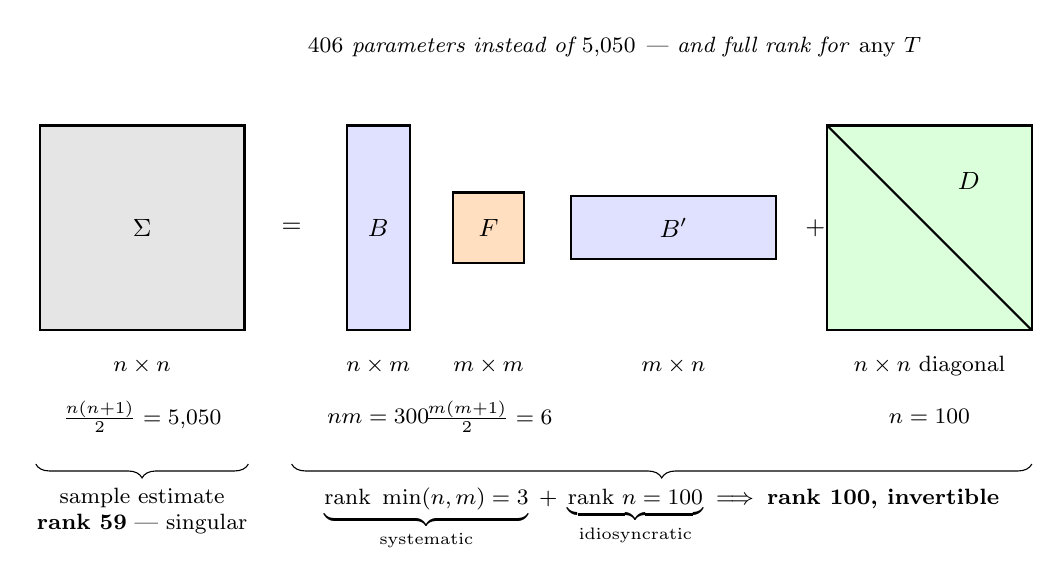
\begin{tikzpicture}[font=\small,
  bx/.style={draw,thick},
  lbl/.style={font=\footnotesize},
  cnt/.style={font=\footnotesize\itshape}]

% Sigma  (n x n)
\node[bx,fill=black!10,minimum width=26mm,minimum height=26mm] (S) at (0,0) {$\Sigma$};
\node[lbl] at (0,-1.75) {$n\times n$};
\node[cnt,align=center] at (0,-2.4) {$\tfrac{n(n+1)}{2}=5{,}050$};

\node at (1.9,0) {$=$};

% B  (n x m)
\node[bx,fill=blue!12,minimum width=8mm,minimum height=26mm] (B) at (3.0,0) {$B$};
\node[lbl] at (3.0,-1.75) {$n\times m$};
\node[cnt] at (3.0,-2.4) {$nm=300$};

% F  (m x m)
\node[bx,fill=orange!25,minimum width=9mm,minimum height=9mm] (F) at (4.4,0) {$F$};
\node[lbl] at (4.4,-1.75) {$m\times m$};
\node[cnt,align=center] at (4.4,-2.4) {$\tfrac{m(m+1)}{2}=6$};

% B'  (m x n)
\node[bx,fill=blue!12,minimum width=26mm,minimum height=8mm] (Bt) at (6.75,0) {$B'$};
\node[lbl] at (6.75,-1.75) {$m\times n$};

\node at (8.55,0) {$+$};

% D  (n x n diagonal)
\node[bx,fill=green!14,minimum width=26mm,minimum height=26mm] (D) at (10.0,0) {};
\draw[thick] (8.7,1.3) -- (11.3,-1.3);
\node at (10.5,0.6) {$D$};
\node[lbl,align=center] at (10.0,-1.75) {$n\times n$ diagonal};
\node[cnt] at (10.0,-2.4) {$n=100$};

% braces
\draw[decorate,decoration={brace,amplitude=5pt,mirror}] (-1.35,-3.0) -- (1.35,-3.0);
\node[lbl,align=center] at (0,-3.6) {sample estimate\\ \textbf{rank 59} --- singular};

\draw[decorate,decoration={brace,amplitude=5pt,mirror}] (1.9,-3.0) -- (11.3,-3.0);
\node[lbl,align=center] at (6.6,-3.7)
  {$\underbrace{\text{rank } \min(n,m)=3}_{\text{systematic}}\;+\;
   \underbrace{\text{rank } n=100}_{\text{idiosyncratic}}
   \;\Longrightarrow\; \textbf{rank 100, invertible}$};

\node[cnt,align=center] at (6.0,2.3)
  {$406$ parameters instead of $5{,}050$ --- and full rank for \emph{any} $T$};
\end{tikzpicture}
\end{document}
